
\chapter*{Cadre général du projet}
\addcontentsline{toc}{chapter}{Cadre général du projet}
\markboth{Cadre général du projet}{Cadre général du projet}
\label{chap:cadreGeneral}
%\minitoc

\section*{Introduction}
Dans ce chapitre, nous nous intéresserons à l'introduction du cadre global du projet et à la description des exigences. Il s'agit en fait d'une introduction de l'organisme d'accueil, suivie d'une motivation et de la présentation du projet. Ensuite, nous présentons l'étude de l'existant et la solution proposée.

\section{Présentation de la société d'accueil}
Acteur indépendant et à dimension internationale, NeoLedge est une société française en forte croissance, qui s'appuie sur un réseau de partenaires privilégiés en Europe, en Amérique du Nord et en Afrique. Éditeur spécialisé dans la gestion électronique de documents, NeoLedge compte à son actif des centaines de clients, des dizaines de milliers d'utilisateurs quotidiens et des millions de documents gérés par ses solutions, dans le secteur public comme dans le secteur privé.

\medskip

Partenaire certifié Gold de Microsoft en ce qui concerne le développement d'applications et les plateformes cloud, NeoLedge accompagne des organisations 
pendant leur transition numérique.
NeoLedge s'appuie depuis ses débuts sur les techniques développées par Microsoft. 

\begin{figure}[!h]
\centering

\includegraphics[width=0.5\textwidth]{neoledge_big_logo.png}
\caption{Logo de NeoLedge}
\label{fig:logoNeoledge}
\end{figure}

\subsection{Historique}

Archimed est un éditeur de logiciels français, créé en 1993 par trois fondateurs (Mongi Zidi, Olivier Walbecq et Eric Ruyffelaere) et dont le siège social est établi à Lille.
\medskip

Archimed est un éditeur indépendant spécialisé dans les logiciels de gestion documentaire depuis près de 25 ans. Elle a étendu son activité ECM ces dernières années à travers l'Afrique, l'Europe et l'Amérique du Nord.

\medskip
Afin d'accompagner son développement à l'international, la société a lancé NeoLedge, une nouvelle marque exclusivement dédiée à ses solutions et activités ECM. Le nom NeoLedge a été inspiré par les " new knowledge " - une nouvelle façon de gérer le contenu, d'optimiser le temps et de gagner en productivité.


\subsection{Produits présentés par NeoLedge }
NeoLedge propose une gamme complète de solutions de gestion électronique de documents (GED) et de gestion de contenus (ECM) pour les entreprises et les administrations.

\medskip
% listr
\begin{itemize}
\item \textbf{ECM Elise} : Pour les entreprises de toutes tailles, qui sont confrontées à une gestion complexe des flux d'informations nécessitant de nombreuses interactions avec des tiers, la solution ECM Elise, éditée par NeoLedge, propose des fonctions automatisées pour la capture des flux multicanaux, la gestion des dossiers et l'orchestration des processus métiers.

\item \textbf{DocFactory} : Pour les entreprises à la recherche d'une solution performante capable de les aider dans leur transformation numérique et leur passage au zéro papier, DocFactory est une solution numérique tout-en-un offrant des fonctions centralisées de numérisation, conversion, et capture de documents électroniques, ainsi que d'export et de signature électronique.\\
Contrairement aux solutions propriétaires ne gérant pas le processus de dématérialisation dans sa globalité, DocFactory permet d'industrialiser l'ensemble des opérations de capture des flux de documents jusqu'à leur intégration dans votre système d'information.



\item \textbf{Illico} : Pour les élus et dirigeants de villes de toutes tailles, engagées dans une politique de transition numérique grâce à des outils innovants qui simplifient leur fonctionnement, illico offre aux citoyens et aux équipes de la ville des services de confiance pour la dématérialisation, le traitement des requêtes, la gestion du courrier et l'automatisation des processus métiers. Contrairement aux solutions en silos ne gérant pas la continuité des processus entre les citoyens et les agents, “illico powered by Elise” est un service illimité, rapide à mettre en œuvre, conçu pour les villes et les réseaux de villes.


\end{itemize}

\subsection{Contexte du projet}
Le présent projet intitulé « Elise Mobile » est réalisé dans le cadre de projet de fin d'études pour l'obtention du diplôme de licence national en technologie d'information au sein de l'Institut Supérieur des Etudes Technologiques de Bizerte.

Ce projet a été réalisé dans la société NeoLedge durant la période s'étalant du 06 février 2022 jusqu'à 28 mai 2022

\subsection{Motivation}
Comme nous l'avons déjà indiqué, la société d'accueil dispose d'une application web de Gestion Électronique de Documents (GED) intitulée Elise et qui est développée avec les technologies Vue.js pour la partie front et C\# pour la partie back fournissant des API Rest et services web SOAP. Cette application est commercialisée depuis presque 20 ans sous plusieurs versions, dont la sixième version actuellement. La conception actuelle de l'application ne permet pas aux utilisateurs d'accéder aux différentes informations (documents) pour les nomades, que ce soit via des smartphones/tablettes sous iOS/Android.
L'objectif de ce projet est alors la mise en place d'une solution mobile responsive du Elise tout en gardant les mêmes exigences fonctionnelles, non fonctionnelles et les expériences utilisateurs. Cette application permettra aux utilisateurs d'Elise d'accéder à leurs profils à travers leurs smartphones/tablettes.

\section{Étude de l'existant}
Dans cette section, nous allons présenter l'étude de l'existant, c'est-à-dire l'étude de l'application Elise actuelle et de ses fonctionnalités.
\subsection{Description de l'existant}
La solution existante de Gestion Électronique de Documents a plusieurs fonctionnalités très utiles pour l'organisation. En effet, une fois le document répertorié, il est possible de le retrouver très facilement avec certains critères de recherche prédéfinis. C'est ainsi qu'un gain de temps considérable se fait ressentir, lorsque nous avions l'habitude de rechercher nos documents papier dans des dizaines de classeurs. En ce qui concerne l'indexation des documents, le système prend en charge une reconnaissance automatique des informations présentes sur ce document et assure ainsi un classement optimisé et automatisé.

Désormais, les entreprises sont toujours à la recherche des solutions permettant de développer et faciliter le travail collaboratif. En effet, chaque collaborateur de la société peut avoir accès ou non à tel ou tel document. C'est ainsi que des processus de validation / modification / lecture peuvent être définis, permettant de favoriser le travail commun, et cela même à distance.

C'est pour cela que NeoLedge a proposé une solution GED qui est Elise.

% elise logo
\begin{figure}[!h]
\centering

\includegraphics[width=0.5\textwidth]{elise_logo.png}
\caption{Logo de Elise}
\label{fig:logoElise}
\end{figure}

Elise est une solution verticalisée capable de prendre en charge tous les flux circulants dans l'organisation (entrants, sortants, internes, etc.), et ce, quel que soit le canal (mail, courrier, etc.). Sa  spécificité réside dans sa capacité à gérer les échanges de l'organisation avec son écosystème (partenaires, fournisseurs, citoyens...) par le biais de l'intégration d'une base de tiers, de métadonnées adaptées (expéditeur/destinataire/dates d'échéances...) et de processus de réponse facilités.

Elise peut ainsi gérer des processus transverses et s'appuie sur une modélisation de l'organigramme de la structure concernée (collectivités, administrations, etc.) pour permettre un paramétrage précis des circuits d'acheminement. Ces circuits peuvent bien entendu être modifiés, à tout moment, en cours de route, pour s'adapter à des cas particuliers, fréquents dans le domaine de la Gestion du courrier.

Un service dans Elise est un élément de structure de l'organigramme représentant un groupement d'utilisateurs et/ou de services subordonnés. Les services peuvent être de plusieurs types :

\begin{itemize}
\item \textbf{Service interne} : service interne non joignable directement par une entité d'une autre instance Elise.
\item \textbf{Service interne joignable} : service interne joignable directement par une entité d'une autre instance Elise.
\item \textbf{Service externe} : service appartenant à une autre instance Elise.
\end{itemize}

L'unité d'organisation dans Elise est un élément de l'organigramme pouvant contenir des utilisateurs et services mais uniquement utilisé dans le but de structurer l'organigramme. Contrairement à un service, il est impossible d'affecter des tâches à une unité d'organisation.

\begin{figure}[!h]
\centering
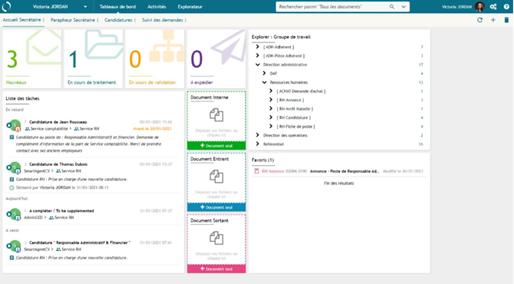
\includegraphics{elise.png}
\caption{Capture d'écran de Elise}
\label{fig:captureElise}
\end{figure}


L'espace de travail Elise est un regroupement de services et d'utilisateurs. Les espaces de travail permettent de rassembler les documents pour lesquels les utilisateurs et services de l'espace de travail ont une tâche à effectuer.

Il existe trois types d'espaces de travail sous Elise :

\begin{itemize}

\item \textbf{Espace de travail par défaut} : Cet espace de travail est composé du service principal d'utilisateur et de lui-même.
\item \textbf{Espaces de travail personnels} : Espaces de travail que l'utilisateur peut créer et configurer lui-même selon ses besoins.
\item \textbf{Espaces de travail de services} : Espaces de travail prédéfinis que l'utilisateur peut ajouter dans leur liste d'espaces de travail pour en faciliter l'accès.
\end{itemize}

Le tableau de bord d'Elise est une partie personnalisable de l'interface qui permet de proposer des vues de l'espace de travail en fonction des besoins. 

Il existe deux types de tableaux de bord sous Elise :

\begin{itemize}
\item \textbf{Tableaux de bord personnels} : que l'utilisateur peut créer, modifier ou supprimer selon ses besoins.
\item \textbf{Tableaux de bords partagés} : prédéfinis et déployés par l'administrateur.
\end{itemize}

Un tableau de bord d'Elise est un ensemble de widgets. Où un widget est un élément de tableau de bord personnalisable afin d'afficher des informations et/ou de créer une interface vers une fonctionnalité de l'application.

Les différents types de widgets sont :

\begin{itemize}

\item \textbf{Widget compteur} : qui définit les nombres des documents selon leurs types existants dans le courrier.
\item \textbf{Widget graphique} : qui représente les statistiques de type de documents.
\item \textbf{Widget liste de documents} : qui définit les documents selon leurs types existants dans le courrier.
\item \textbf{Widget liste des tâches} : qui définit les tâches affectées aux utilisateurs.
\item \textbf{Widget note} : qui définit les notes de l'utilisateur.
\item \textbf{Widget nouveau document} : qui permet à l'utilisateur d'ajouter un document.
\item \textbf{Widget page web}
\item \textbf{Widget vue dynamique}
\item \textbf{Widget raccourci} : qui est un raccourci à un document ou à un site web.

\end{itemize}

Dans Elise, un document correspond à un enregistrement complet. Un document contient les éléments suivants :

\begin{itemize}
\item \textbf{Propriétés du document} : Les propriétés sont des données contenant les informations associées à un document.
\item \textbf{Fichiers} : Fichiers numériques liés au document et qui sont éditables par les utilisateurs.
\item \textbf{Les tâches} : Les tâches sont des actions à effectuer sur des documents.
\item \textbf{Un processus} : est un ensemble de tâches définissant les actions à réaliser sur un document.
\item \textbf{Les liens} : Propriétés de type URL qui sont ajoutées soit par un automate soit manuellement.
\item \textbf{Historique des événements} : Les événements gardent la trace de toutes les actions effectuées sur le document.
\end{itemize}

Les différents états du document sont les suivants :

\begin{itemize}

\item \textbf{Sans affectation} : État des documents qui ont été créés mais pour lesquels l'ensemble des propriétés obligatoires n'est pas renseigné et/ou aucune tâche n'est encore attribuée. (Cas documents numérisés non encore enregistrés)
\item \textbf{Préparé} : État des documents pour lesquels l'ensemble des propriétés obligatoires est renseigné et au moins une tâche est attribuée. Le changement d'état depuis l'état « Préparé » vers l'état « en cours de traitement » se fait en distribuant le document.
\item \textbf{En circulation} : État des documents pour lesquels il y a des tâches actives en cours de traitement et qui n'ont pas été clôturés. Le changement d'état depuis l'état « En circulation » vers « Clôturé » se fait en clôturant le document.
\item \textbf{Clôturé} : État des documents pour lesquels toutes les tâches qui devaient être effectuées sont terminées et qui ont été clôturés. Le changement d'état depuis l'état « Clôturé » vers l'état « Archivé » se fait en archivant le document.
\item \textbf{Archivé} : État des documents pour lesquels la période d'utilité dans Elise est terminée et qui ne nécessitent donc plus d'être accessibles par les utilisateurs.

\end{itemize}

NeoLedge a une version actuelle du Elise Mobile qui se trouve déjà sur le marché du mobile hébergée dans Play store et App store.

% capture d'ecran elimse mobile actuelle
\begin{figure}[!h]
\centering
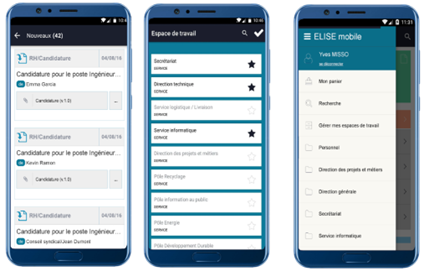
\includegraphics{eliseMobile.png}
\caption{Capture d'écran de Elise Mobile}
\label{fig:captureEliseMobile}
\end{figure}

Elise Mobile est une application mobile pour plateformes iOS et Android :

\begin{itemize}
\item \textbf{Simple à utiliser} : Elise Mobile est une application intuitive et facile à utiliser. Elle permet de gérer les documents et les tâches depuis n'importe quel endroit et à tout moment.
\item \textbf{Facile à déployer} : Elise Mobile est une application qui ne nécessite pas de configuration particulière. Elle est disponible sur les plateformes iOS et Android.
\item \textbf{Au ROI immédiat} : Elise Mobile permet de gagner du temps et de l'argent en permettant aux utilisateurs de gérer leurs documents et leurs tâches.
\end{itemize}

Elle a été développée en Xamarin avec Backend en Asp.Net Core 4 depuis le 10 octobre 2018. Elle est en version 1.1.6 jusqu'à présent.

Avec Elise Mobile, les utilisateurs de la solution de Gestion électronique de Contenu Elise peuvent :

\begin{itemize}
%   	Collaborer à distance :
% o	Accéder à l'ensemble de leurs tâches selon leur état de traitement (Nouveaux, En cours, Terminés...)
% o	Superviser leurs processus métiers
% o	Effectuer des recherches dans la base documentaire
% 	Décider en quelques instants
% o	Traiter leurs tâches
% o	Valider/Refuser rapidement les actions demandées
% o	Demander/Transférer des tâches
% o	Respecter les délais
% 	Superviser leurs espaces de travail
% o	Accéder aux espaces de travail de leurs différents services
% o	Visualiser les tâches en cours o Contrôler les échéances

\item \textbf{Collaborer à distance} : 
  \begin{itemize}
  \item Accéder à l'ensemble de leurs tâches selon leur état de traitement (Nouveaux, En cours, Terminés...)
  \item Superviser leurs processus métiers
  \item Effectuer des recherches dans la base documentaire
  \end{itemize}
\item \textbf{Décider en quelques instants} :
  \begin{itemize}
  \item Traiter leurs tâches
  \item Valider/Refuser rapidement les actions demandées
  \item Demander/Transférer des tâches
  \item Respecter les délais
  \end{itemize}
\item \textbf{Superviser leurs espaces de travail} :
  \begin{itemize}
    \item Accéder aux espaces de travail de leurs différents services
    \item Visualiser les tâches en cours o Contrôler les échéances
  \end{itemize}
\end{itemize}

\subsection{Critique de l'existant}
L'étude de l'application existante nous a permis de porter des jugements objectifs afin de projeter de fournir ainsi un système plus fiable.

Parmi les lacunes rencontrées, nous citons :
\begin{itemize}
  % \item Elise est une solution développée de base en ASP. Net Back et front de l'ancienne version d'Asp. Net c'est pour cela l'application actuelle est non responsive et c'est à partir de la version 6 de Elise que NeoLedge a décidé de migrer le front vers les nouvelles technologies. 
  % \item Elise utilise une base de données locale qui est SIMWebPack et qui est une solution proposée par NeoLedge pour enregistrer les documents sous la forme de XML.
  \item La version actuelle d'Elise mobile ne répond pas aux besoins des utilisateurs par rapport à Elise web ce qui invoque de mauvaises expériences utilisateurs.
  \item La version actuelle d'Elise mobile ne renferme pas toutes les fonctionnalités du Elise version web.
\end{itemize}

\subsection{Solution proposée}
Notre solution consiste à mettre en place une solution responsive de Elise qui offre les mêmes fonctionnalités que la version web actuelle d'Elise tout en gardant les mêmes interfaces pour améliorer l'expérience d'utilisateur. Parmi les fonctionnalités qu'on va traiter, on peut citer :

\begin{itemize}
  \item Connecter un utilisateur de Elise à son profil
  \item Consulter les espaces de travail
  \item	Consulter les tableaux de bord
  \item	Créer un nouveau document
  \item Accéder à un document
  \item Rechercher un document / un service ou un utilisateur spécifique
  \item Signer des documents
  \item	Gestion des documents
  \begin{itemize}
    \item Possibilité d'approuver et de signer des documents.
    \item Signature possible en utilisant des signatures antérieures ou manuellement.
    \item Possibilité d'utiliser des signatures électroniques avancées.
  \end{itemize}
  \item Notifications push : Possibilité de recevoir des notifications push pour les mises à jour de documents ou les tâches à effectuer.
\end{itemize}

\section{Étude technique}
\subsection{Architecture système}
Elise est une solution d'architecture architecture 3 tiers, illustrée par la figure ci-dessous 
% image architecture_elise
\begin{figure}[H]
  \centering
  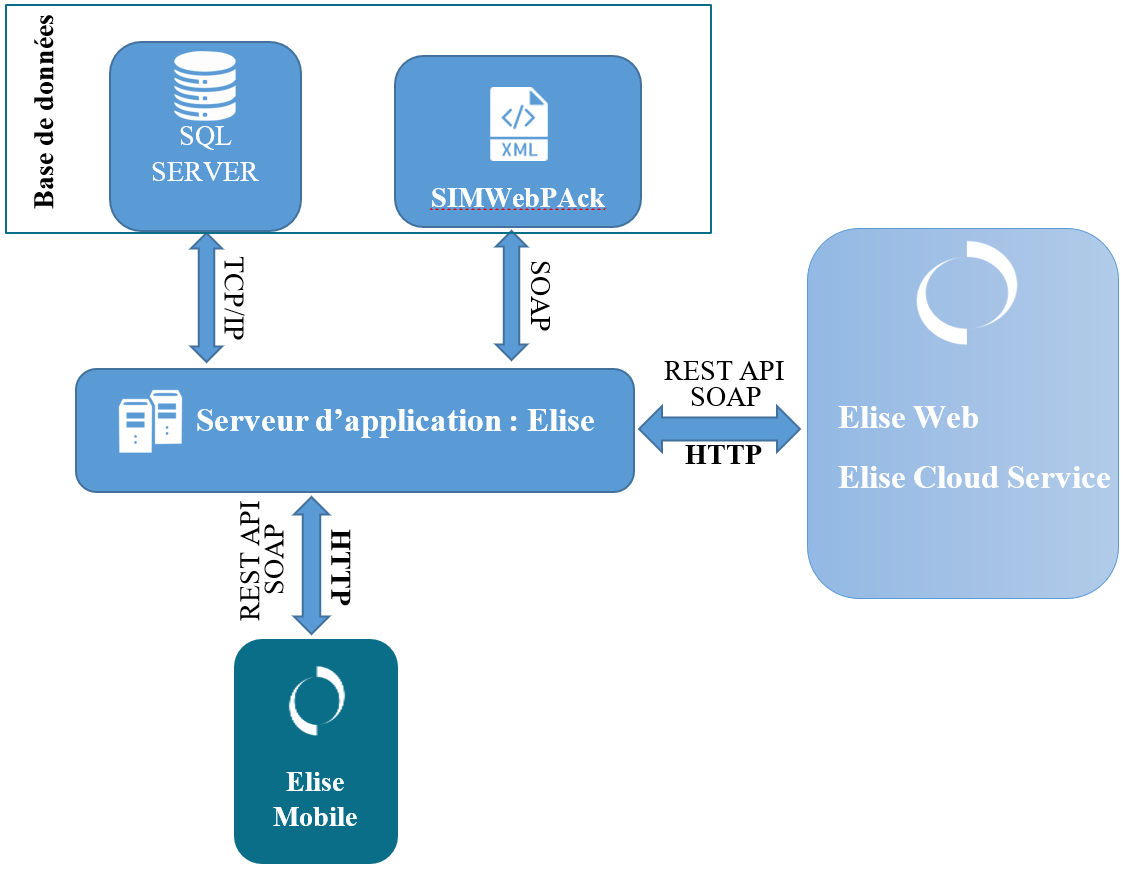
\includegraphics[width=0.8\textwidth]{architecture_elise}
  \caption{Architecture Elise}
  \label{fig:architecture_elise}
\end{figure}
Cette architecture est composée de trois couches (3 tiers) :

\subsubsection{La couche client (ou la couche présentation)}
C'est la couche frontale de l'application. Elle comprend l'interface utilisateur. Pour notre solution c'est l'application Elise web et les autres applications de ECS : Elise Cloud Service. Et nous allons intégrons notre application mobile à cette couche. Ou toutes les applications de cette couche communiquent avec les autres couches avec des appels web services.

\subsubsection{La couche applicative}
Contient la logique métier fonctionnelle qui pilote les fonctionnalités essentielles d'une application. Dans notre cas, c'est le serveur d'application Elise.

\subsubsection{	La couche d'accès aux données}
Elle contient les données de l'application. Pour notre solution nous avons deux types de base de données ; une base de données relationnelles et une base de données Xml.

Cette architecture nous offre la séparation entre l'interface utilisateur, la logique métier et la couche de stockage de données. Cela donne une plus grande flexibilité aux équipes de développement en leur permettant de mettre à jour une partie spécifique d'une application indépendamment des autres parties.

\section{Méthodologie de gestion de projet}
Avec les progrès en technologie de l'information et les investissements dans les infrastructures, beaucoup de méthodes de gestion de projet ont vu le jour. Certes, ces méthodes jouent un rôle primordial dans la réussite ou l'échec d'un projet, d'où le choix, représente une décision importante pour les entreprises. Dans cette partie, nous allons expliquer notre choix de la méthode. Il existe en fait deux grandes familles de méthodes de la gestion du projet : les méthodes dites classiques et les méthodes agiles. On privilégiera plutôt les méthodes classiques lorsqu'on a une idée précise du projet, avec un planning bien détaillé et où on a anticipé tous les risques possibles. Quant aux méthodes Agiles, on les choisira plutôt pour les gros projets, celles-ci permettent une meilleure adaptabilité, visibilité et gestion des risques. On privilégiera également les méthodes Agiles pour les projets où il n'y a pas de documents détaillés, ou quand le client est indécis. Le client pourra alors voir l'évolution du projet et l'adapter à ses besoins sans pour autant vous obliger à recommencer tout le travail que vous avez fourni depuis le début. Elles sont menées dans un esprit collaboratif et elles s'adaptent aux approches incrémentales. Elles engendrent des produits de haute qualité tout en tenant compte de l'évolution des besoins du client.

\subsection{Choix méthodologique}
Notre choix méthodologique et en convenance à notre projet, nous avons opté pour l'utilisation du framework Scrum. C'est en fait le framework le plus utilisé, le plus éprouvé, documenté et supporté. Il s'agit d'un cadre de travail en équipe pluridisciplinaire permettant de répondre à des problèmes complexes et changeants, centré sur l'architecture.
\subsection{Pourquoi Scrum}
Dans le cadre de notre projet et afin d'assurer le bon déroulement des différentes phases de ce dernier, nous avons opté pour le framework agile Scrum pour la conception et le développement de notre système pour des raisons bien déterminées. En effet, le framework Scrum s'adapte parfaitement à la décomposition de notre projet de fin d'études.

Il se base sur les avantages suivants :

\begin{itemize}
  \item Plus de souplesse et de réactivité.
  \item Grande capacité d'adaptation au changement grâce à des itérations courtes.
  \item Satisfaire au mieux les besoins du client.
\end{itemize}



SCRUM est une méthodologie agile qui consiste à avoir une équipe soudée orientant le projet au fil de son avancement afin d'atteindre un but. Cette approche est à la fois dynamique et productive, engendre la réalisation des fonctionnalités par itération en incluant la participation du client. Chaque itération peut durer de deux à quatre semaines, à la fin de chaque sprint un produit fonctionnel doit être livré. En effet, Scrum définit trois rôles qui sont :

\begin{itemize}
  \item \textbf{Product Owner }(Le gestionnaire de produit):
  Le responsable du produit de l'équipe projet client et il représente les utilisateurs finaux. C'est lui qui va définir et prioriser la liste des fonctionnalités du produit et choisir la date et le contenu de chaque sprint sur la base des valeurs (charges) qui lui sont communiquées par l'équipe.
  \item \textbf{Scrum Master} (Le maître de Scrum):
  Véritable facilitateur sur le projet, il veille à ce que chacun puisse travailler au maximum de ses capacités en éliminant les obstacles et en protégeant l'équipe des perturbations extérieures.
  \item \textbf{L'équipe de développement} (L'équipe de projet):
  L'équipe de réalisation contient au minimum deux développeurs. Elle regroupe tous les rôles habituellement nécessaires à un projet, à savoir l'architecte, le concepteur, le développeur, le testeur, etc.
\end{itemize}

\begin{figure}[!h]
  \centering
  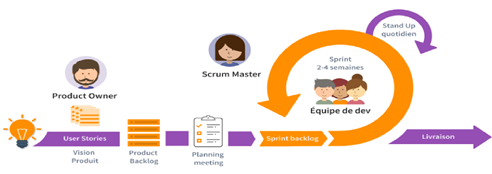
\includegraphics{cycle_de_vie_scrum.png}
  \caption{Cycle de vie Scrum}
  \label{fig:cycle_de_vie_scrum}
\end{figure}

\section{Environnement de développement}
Avant d'entamer la mise en œuvre de notre projet, nous allons d'abord décrire l'environnement et les outils de travail que nous utiliserons. Nous commencerons par définir l'environnement matériel, suivi de l'environnement logiciel. Enfin, nous présenterons les différents langages et frameworks que nous utiliserons dans le cadre de ce projet.

\subsection{Environnement matériel}

\begin{table}[H]
  \centering
  \begin{center}
    \begin{tabular}{|p{0.3\linewidth}|p{0.6\linewidth}|}
      \hline
      Environnement matériel & Description \\
      \hline
      
      \begin{minipage}{\linewidth}
        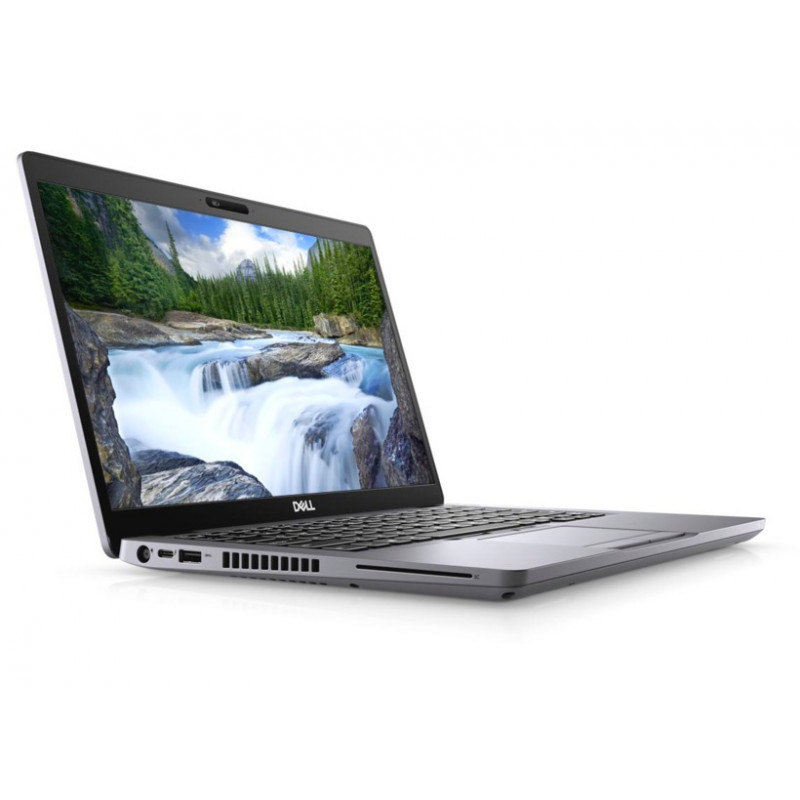
\includegraphics[width=\linewidth]{pc.jpg}
      \end{minipage} &
      \begin{minipage}{\linewidth}
        \vspace{0.2cm}
        \textbf{PC DELL Latitude 5510}
        \begin{itemize}
          \item \textbf{Quantité} : 2
          \item \textbf{Processeur} : Intel Core i7-10610U 
          \item \textbf{Mémoire} : 16 Go DDR4 
          \item \textbf{Stockage} : 512Go SSD 
          \item \textbf{Carte graphique} : NVIDIA GeForce MX250 
          \item \textbf{Système d'exploitation} : Windows 10 
        \end{itemize}
        \vspace{0.2cm}
      \end{minipage} \\
      \hline
      \begin{minipage}{\linewidth}
        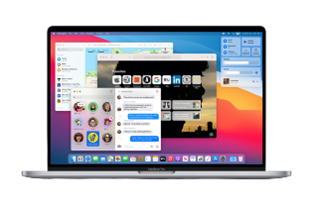
\includegraphics[width=\linewidth]{macbookpro}
      \end{minipage} &
      \begin{minipage}{\linewidth}
        \vspace{0.2cm}
        \textbf{MacBook Pro}
        \begin{itemize}
          \item \textbf{Processeur} : Puce Apple M1 - CPU 8 
          \item \textbf{Mémoire} : 8 Go DDR4
          \item \textbf{Stockage} : 256 Go SSD
          \item \textbf{Système d'exploitation} : macOS Big Sur 
        \end{itemize}
        \vspace{0.2cm}
      \end{minipage} \\


      \hline
      \begin{minipage}{\linewidth}
        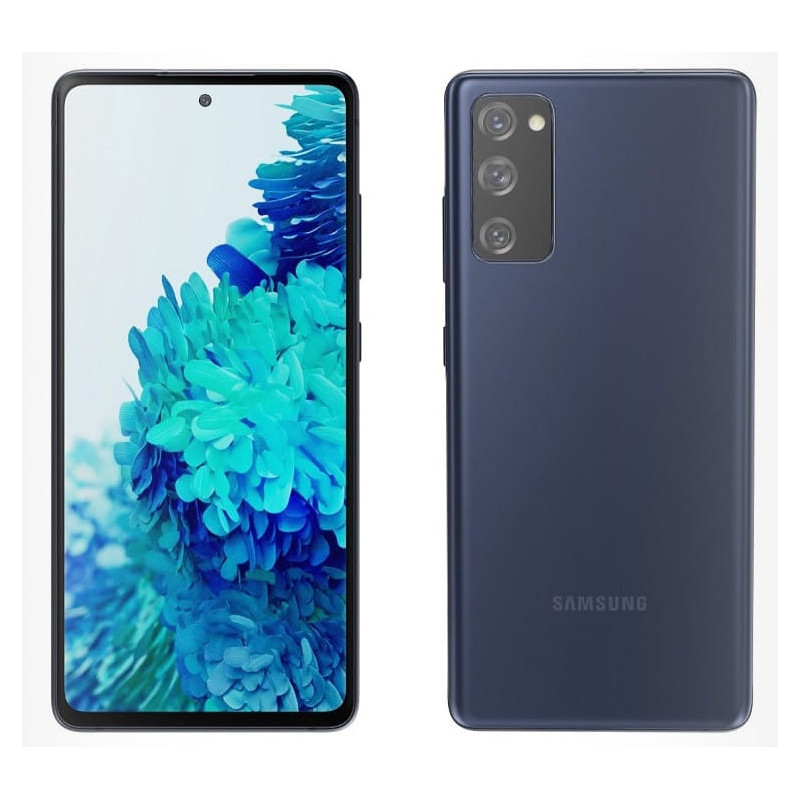
\includegraphics[width=\linewidth]{samsungs20}
      \end{minipage} &
      \begin{minipage}{\linewidth}
        \vspace{0.2cm}
        \textbf{Samsung Galaxy S20 FE 5G}
        \begin{itemize}
          \item \textbf{Processeur} : Cortex-A55 
          \item \textbf{Mémoire} : 12 Go 
          \item \textbf{Stockage} : 128 Go
          \item \textbf{Système d'exploitation} : Android 13
        \end{itemize}
        \vspace{0.2cm}
      \end{minipage} \\

      \hline
      \begin{minipage}{\linewidth}
        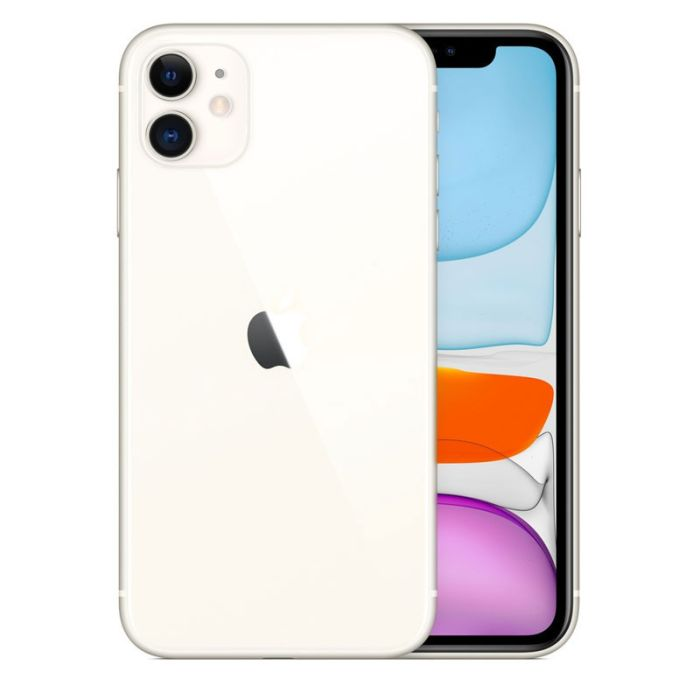
\includegraphics[width=\linewidth]{iphone11}
      \end{minipage} &
      \begin{minipage}{\linewidth}
        \vspace{0.2cm}
        \textbf{Iphone 11}
        \begin{itemize}
          \item \textbf{Processeur} : Apple A13 Bionic
          \item \textbf{Mémoire} : 4 Go
          \item \textbf{Stockage} : 64 Go
          \item \textbf{Système d'exploitation} : iOS 16.3
        \end{itemize}
        \vspace{0.2cm}
      \end{minipage} \\

      \hline
      
      

    \end{tabular}

  \caption{Environnement matériel}
  \label{tab:environnement_materiel}
  \end{center}
\end{table}

\subsection{Environnement logiciel}
Au cours de cette section, nous dresserons une liste des outils utilisés pour étudier et mettre en place notre application tout au long du projet.

\begin{itemize}
  \item \textbf{Windows 10} :\\
  \begin{minipage}{\linewidth}
    \begin{wrapfigure}{l}{0.125\textwidth}
      \vspace{-0.5cm}
      
\includegraphics[width=1\linewidth]{win10.jpg} 
    \end{wrapfigure}
    Windows 10 est un système d'exploitation de Microsoft. Cette nouvelle
version introduit plusieurs changements importants. Elle est la
première à fonctionner sur tou
tes les plateformes existantes.
    \end{minipage}

    \vspace{0.5cm}

  \item \textbf{Visual Studio Code} :\\
  \begin{minipage}{\linewidth}
    \begin{wrapfigure}{l}{0.125\textwidth}
      \vspace{-0.5cm}
      
\includegraphics[width=0.9\linewidth]{vscode.png} 
    \end{wrapfigure}
    Un éditeur de code extensible développé par Microsoft pour Windows, Linux et macOS. Les fonctionnalités incluent
     la prise en charge du débogage, la mise en évidence de la syntaxe, la complétion intelligente du code, les snippets, la refactorisation du code et Git intégrer.
  \end{minipage}
    
  \item \textbf{XCode} :\\
  \begin{minipage}{\linewidth}
    \begin{wrapfigure}{l}{0.125\textwidth}
      \vspace{-0.5cm}
      
\includegraphics[width=0.9\linewidth]{xcode} 
    \end{wrapfigure}
    Xcode est un environnement de développement pour macOS, ainsi que pour iOS, watchOS et tvOS. 
    \end{minipage}

    \vspace{0.5cm}
    \item \textbf{Android Studio} :\\
    \begin{minipage}{\linewidth}
      \begin{wrapfigure}{l}{0.125\textwidth}
        \vspace{-0.5cm}
        
\includegraphics[width=0.9\linewidth]{android.png} 
      \end{wrapfigure}
      Android Studio est un environnement de développement intégré (IDE) pour le développement d'applications Android. Il est basé sur IntelliJ IDEA et est développé par Google.
    \end{minipage}

    \vspace{0.5cm}

    \item \textbf{Postman} :\\
    \begin{minipage}{\linewidth}
      \begin{wrapfigure}{l}{0.125\textwidth}
        \vspace{-0.5cm}
        
\includegraphics[width=0.9\linewidth]{postman.jpg} 
      \end{wrapfigure}
      Postman est un outil de développement de logiciels qui permet de tester et de déboguer des API. Il permet de créer des requêtes HTTP et de les envoyer à un serveur. Il permet également de créer des collections de requêtes et de les organiser en dossiers.
    \end{minipage}

    \vspace{0.5cm}
    \item \textbf{Git} :\\
    \begin{minipage}{\linewidth}
      \begin{wrapfigure}{l}{0.125\textwidth}
        \vspace{-0.5cm}
        
\includegraphics[width=0.9\linewidth]{git.jpg} 
      \end{wrapfigure}
      Git est un logiciel de gestion de versions décentralisé. Il permet de gérer les versions d'un projet informatique et de collaborer avec d'autres développeurs.
    \end{minipage}
    

    \vspace{0.5cm}
    \item \textbf{Azure DevOps} :\\
    \begin{minipage}{\linewidth}
      \begin{wrapfigure}{l}{0.125\textwidth}
        \vspace{-0.5cm}
        
\includegraphics[width=0.9\linewidth]{AzureDevOps.png} 
      \end{wrapfigure}
      Azure DevOps est un ensemble d'outils de développement logiciel en tant que service (SaaS) fourni par Microsoft. Il fournit des services de gestion de projets, de gestion de code source, de gestion de tests et de gestion de la qualité du logiciel.
    \end{minipage}

    \vspace{0.5cm}
    \item \textbf{Figma} :\\
    \begin{minipage}{\linewidth}
      \begin{wrapfigure}{l}{0.125\textwidth}
        \vspace{-0.8cm}
        
\includegraphics[width=0.9\linewidth]{figma.jpg} 
      \end{wrapfigure}
      Figma est un outil de conception graphique. Il permet de créer des maquettes de sites web et d'applications mobiles.
    \end{minipage}

    \vspace{0.5cm}
    \item \textbf{Draw.io} :\\
    \begin{minipage}{\linewidth}
      \begin{wrapfigure}{l}{0.125\textwidth}
        \vspace{-0.5cm}
        
\includegraphics[width=0.9\linewidth]{drawio.png} 
      \end{wrapfigure}
      Draw.io est un logiciel de dessin graphique multiplateforme gratuit et open source développé en HTML5 et JavaScript. Son interface peut être utilisée pour créer tous types de diagrammes.
    \end{minipage}

    \vspace{0.5cm}
    \item \textbf{Microsoft Teams} :\\
    \begin{minipage}{\linewidth}
      \begin{wrapfigure}{l}{0.125\textwidth}
        \vspace{-0.5cm}
        
\includegraphics[width=0.9\linewidth]{teams.png} 
      \end{wrapfigure}
      Microsoft Teams est un logiciel de messagerie instantanée et de collaboration en ligne développé par Microsoft. Il permet de créer des salons de discussion, de partager des fichiers et de collaborer en temps réel.
    \end{minipage}

    \vspace{0.5cm}
    \item \textbf{Latex} :\\
    \begin{minipage}{\linewidth}
      \begin{wrapfigure}{l}{0.125\textwidth}
        \vspace{-0.5cm}
        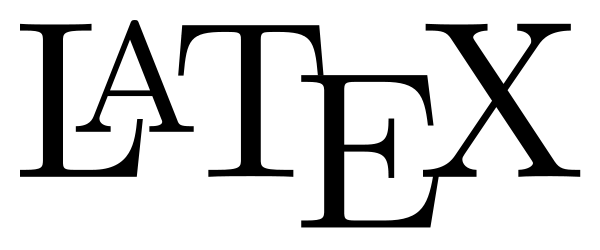
\includegraphics[width=0.9\linewidth]{latex.png} 
      \end{wrapfigure}
      LaTeX est un langage de description de documents. Il permet de créer tous types de documents. Il est utilisé pour la rédaction de livres, de rapports, de thèses, de journaux, de présentations, de documents techniques, etc.
    \end{minipage}

    \vspace{0.5cm}
    \item \textbf{NodeJs} :\\
    \begin{minipage}{\linewidth}
      \begin{wrapfigure}{l}{0.125\textwidth}
        \vspace{-0.5cm}
        
\includegraphics[width=0.9\linewidth]{nodejs.png}
      \end{wrapfigure}
      Node.js est une plateforme logicielle libre en JavaScript, orientée vers les applications réseau évènementielles hautement concurrentes.
    \end{minipage}
    \vspace{0.5cm}

    \item \textbf{Firebase} :\\
    \begin{minipage}{\linewidth}
      \begin{wrapfigure}{l}{0.125\textwidth}
        \vspace{-0.5cm}
        
\includegraphics[width=0.9\linewidth]{firebase} 
      \end{wrapfigure}
      Firebase est un ensemble de services d'hébergement pour n'importe quel type d'application.
      Il propose d'héberger en NoSQL et en temps réel des bases de données, du contenu, et des notifications, etc.
    \end{minipage}
  \end{itemize}


  \subsection{Technologies utilisées}

  \begin{itemize}
    \item \textbf{Ionic} :\\
    \begin{minipage}{\linewidth}
      \begin{wrapfigure}{l}{0.125\textwidth}
        \vspace{-0.5cm}
        
\includegraphics[width=0.9\linewidth]{ionic.png} 
      \end{wrapfigure}
      Ionic est un UI toolkit open source pour la création d'applications mobiles performantes et de haute qualité à l'aide de technologies web telles que HTML, CSS et JavaScript, avec des intégrations pour des frameworks populaires tels que Angular, React et Vue.
    \end{minipage}
  
    \vspace{0.5cm}
  
    \item \textbf{Vue3} :\\
    \begin{minipage}{\linewidth}
      \begin{wrapfigure}{l}{0.125\textwidth}
        \vspace{-0.5cm}
        
\includegraphics[width=0.9\linewidth]{vue.png} 
      \end{wrapfigure}
      Vue.js est un framework JavaScript open source pour la création d'interfaces utilisateur et d'applications web monopages.
    \end{minipage}
  
    \vspace{0.5cm}
  
    \item \textbf{Capacitor} :\\
    \begin{minipage}{\linewidth}
      \begin{wrapfigure}{l}{0.125\textwidth}
        \vspace{-0.5cm}
        
\includegraphics[width=0.9\linewidth]{capacitor.png} 
      \end{wrapfigure}
      Capacitor est un runtime natif open source pour la création d'applications Web natives. Il permet de créer des applications iOS, Android et des applications Web progressives multiplateformes à l'aide de JavaScript, HTML et CSS.
    \end{minipage}
  
    \vspace{0.5cm}
  
    \item \textbf{Typescript} :\\
    \begin{minipage}{\linewidth}
      \begin{wrapfigure}{l}{0.125\textwidth}
        \vspace{-0.5cm}
        
\includegraphics[width=0.9\linewidth]{typescript.png} 
      \end{wrapfigure}
      TypeScript est un langage de programmation libre et open source développé par Microsoft. Il est un sur-ensemble de JavaScript, c'est-à-dire qu'il ajoute des fonctionnalités à ce dernier.
    \end{minipage}
  
    \vspace{0.5cm}
  
    \item \textbf{Javascript} :\\
    \begin{minipage}{\linewidth}
      \begin{wrapfigure}{l}{0.125\textwidth}
        \vspace{-0.5cm}
        
\includegraphics[width=0.9\linewidth]{javascript.png} 
      \end{wrapfigure}
      JavaScript est un langage de programmation de scripts principalement employé dans les pages web interactives et à ce titre est une partie essentielle des applications web.
    \end{minipage}

    \vspace{0.5cm}
  
    \item \textbf{Pinia} :\\
    \begin{minipage}{\linewidth}
      \begin{wrapfigure}{l}{0.125\textwidth}
        \vspace{-0.5cm}
        
\includegraphics[width=0.9\linewidth]{pinia.png} 
      \end{wrapfigure}
      Pinia est une bibliothèque de magasin et un framework de gestion d'état pour Vue.js. Conçu principalement pour créer des applications Web frontales, il utilise une syntaxe déclarative et propose sa propre API de gestion d'état.
    \end{minipage}
    
    \vspace{0.5cm}
  
    \item \textbf{PlantUML} :\\
    \begin{minipage}{\linewidth}
      \begin{wrapfigure}{l}{0.125\textwidth}
        \vspace{-0.5cm}
        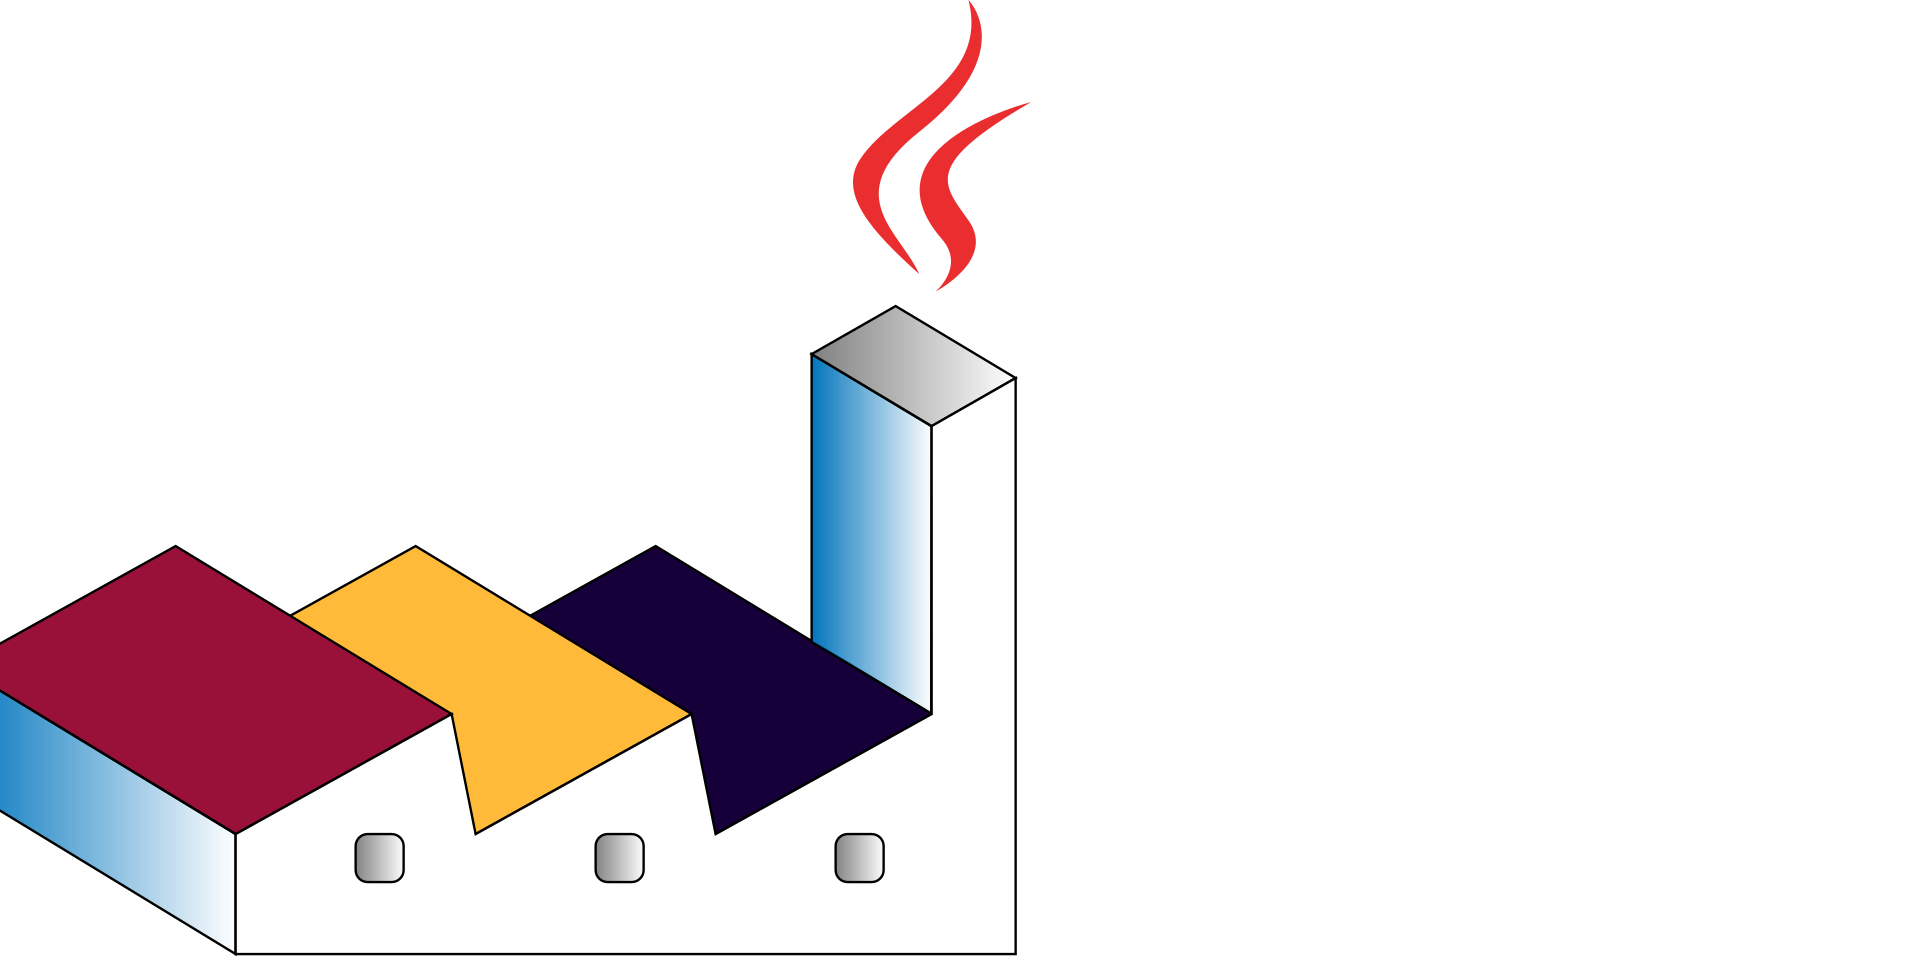
\includegraphics[width=0.9\linewidth]{plantuml.png} 
      \end{wrapfigure}
      PlantUML est un outil open-source permettant aux utilisateurs de créer des diagrammes à partir d'un langage de texte simple.
    \end{minipage}

    \item \textbf{Jest} :\\
    \begin{minipage}{\linewidth}
      \begin{wrapfigure}{l}{0.125\textwidth}
        \vspace{-0.5cm}
        
\includegraphics[width=0.9\linewidth]{jest.png} 
      \end{wrapfigure}
      Jest est un framework de test JavaScript construit sur Jasmine et maintenu par Meta. Il a été conçu et construit en mettant l'accent sur la simplicité et la prise en charge des grandes applications Web.
    \end{minipage}
  
    \vspace{0.5cm}
    \item \textbf{Express} :\\
    \begin{minipage}{\linewidth}
      \begin{wrapfigure}{l}{0.125\textwidth}
        \vspace{-0.5cm}
        
\includegraphics[width=0.9\linewidth]{express.png}
      \end{wrapfigure}
      Express est un framework pour construire des applications web basées sur Node.js. C'est de fait le framework standard pour le développement de serveur en Node.js. 
    \end{minipage}

  
  \end{itemize}



\section*{Conclusion}
Au cours de ce chapitre qui constitue une étape primordiale pour fixer les repères de notre projet. Nous avons présenté l'organisme d'accueil et les attentes du projet. En effet, nous avons mené une étude de l'existant afin de mieux cerner les fonctionnalités de notre solution révélant les limites de la solution existante. Nous avons également déterminé le cadre du travail ainsi que la méthodologie à emprunter lors de ce projet.

Dans le chapitre qui suit nous allons décrire la conception de l'application en détaillant ses spécifications, ses acteurs et ses différents diagrammes de cas d'utilisation, de séquences, de classes, et d'activités.


